%%%%%%%%%%%%%%%%%%%%%%%%%%%%%%%%%%%%%%%%%%%%%%%%%%%%%%%%%%%%%%%%%%%%%%%%%%%%%%%
%%                                                                           %%
%%   Dr Derek Harter                                                         %%
%%   Profesor, Department of Computer Science                                %% 
%%   Texas A&M University - Commerce, USA                                    %%
%%                                                                           %%
%%%%%%%%%%%%%%%%%%%%%%%%%%%%%%%%%%%%%%%%%%%%%%%%%%%%%%%%%%%%%%%%%%%%%%%%%%%%%%%
%%%%     SETTING STARTS - DO NOT CHANGE Unless your TeX setting require so   %%
%%%%%%%%%%%%%%%%%%%%%%%%%%%%%%%%%%%%%%%%%%%%%%%%%%%%%%%%%%%%%%%%%%%%%%%%%%%%%%%
%%----------------------------------------------------------------------------------
% DO NOT Change this. It is the required setting letterpaper page, 11pt, onside print, book style
%%----------------------------------------------------------------------------------
\documentclass[letterpaper,11pt,oneside]{book}

%%-------------------------------------
%% Page margin settings - % half inch margin all sides (recommended)
%%-------------------------------------
\usepackage[margin=1.2in]{geometry} 

%%-------------------------------------
%% Font settings - % CM San or Ariel (recommended)
%%-------------------------------------
% Switch the following two line off: to revert back to default LaTex font (NOT recommended)
\usepackage{amsfonts}
\renewcommand*\familydefault{\sfdefault}

%%-------------------------------------
%% Math/Definition/Theorem/Algorithm packages settings 
%%-------------------------------------
\usepackage[cmex10]{amsmath}
\usepackage{amssymb}
\usepackage{amsthm}
\newtheorem{mydef}{Definition}
\newtheorem{mytherm}{Theorem}

%%-------------------------------------
%% Algorithms/Code Listing environment settings  - 
%% Please do not change these settings
%%-------------------------------------
\usepackage{algorithm}
\usepackage{algpseudocode}
\renewcommand{\algorithmicrequire}{\textbf{Input:}}
\renewcommand{\algorithmicensure}{\textbf{Output:}}
\usepackage[utf8]{inputenc}
\usepackage{listings}
\usepackage{xcolor}
\definecolor{codegreen}{rgb}{0,0.6,0.1}
\definecolor{codegray}{rgb}{0.5,0.5,0.5}
\definecolor{codeblue}{rgb}{0.10,0.00,1.00}
\definecolor{codepurple}{rgb}{0.58,0,0.82}
\definecolor{backcolour}{rgb}{1.0,1.0,1.0}

\lstdefinestyle{mystyle}{
    backgroundcolor=\color{backcolour},   
    commentstyle=\color{codegreen},
    keywordstyle=\color{codeblue},
    numberstyle=\tiny\color{codegray},
    stringstyle=\color{codepurple},
    basicstyle=\ttfamily\footnotesize,
    breakatwhitespace=false,         
    breaklines=true,                 
    captionpos=b,                        
    keepspaces=true,                 
    numbers=left,                    
    numbersep=5pt,                  
    showspaces=false,                
    showstringspaces=false,
    showtabs=false,                  
    tabsize=2,
    frame=none
}
\lstset{style=mystyle}

%%-------------------------------------
%% Graphics/Figures environment settings
%%-------------------------------------
\usepackage{graphicx}
\usepackage{subfigure}
\usepackage{caption}
\usepackage{lipsum}

%%-------------------------------------
%% Table environment settings
%%-------------------------------------
\usepackage{multirow}
\usepackage{rotating}
\usepackage{makecell}
\usepackage{booktabs}
%\usepackage{longtable,booktabs}

%%-------------------------------------
%% List of Abbreviations settings
%%-------------------------------------
\usepackage{enumitem}
\newlist{abbrv}{itemize}{1}
\setlist[abbrv,1]{label=,labelwidth=1in,align=parleft,itemsep=0.1\baselineskip,leftmargin=!}

%%-------------------------------------
%% Bibliography/References settings   - Harvard Style was used in this report
%%-------------------------------------
\usepackage[hidelinks]{hyperref}
\usepackage[comma,authoryear]{natbib}
\renewcommand{\bibname}{References} % DO NOT remove or switch of 

%%-------------------------------------
%% Appendix settings     
%%-------------------------------------
\usepackage[toc]{appendix}
%%%%%%%%%%%%%%%%%%%%%%%%%%%%%%%%%%%%%%%%%%%%%%%%%%%%%%%%%%%%%%%%%%%%%%%%%%%%%%%%%%%%%%%
%%%%                     SETTING ENDS                                            %%%%%%
%%%%%%%%%%%%%%%%%%%%%%%%%%%%%%%%%%%%%%%%%%%%%%%%%%%%%%%%%%%%%%%%%%%%%%%%%%%%%%%%%%%%%%%
\begin{document}

    \captionsetup[figure]{margin=1.5cm,font=small,name={Figure},labelsep=colon}
    \captionsetup[table]{margin=1.5cm,font=small,name={Table},labelsep=colon}
    \SetLipsumDefault{1}
    
    \frontmatter
    
    \begin{titlepage}      
        \begin{center}
            
\includegraphics[width=3cm]{figures/tamuc-logo.png}\\[0.5cm]
            {\LARGE Texas A\&M University - Commerce\\[0.5cm]
            Department of Computer Science}\\[2cm]
			%{\color{blue} \rule{\textwidth}{1pt}}
			
			% -------------------------------
			% You need to edit some details here
			% -------------------------------  
            \linespread{1.2}\huge {
                %%%%%%%%%%%%%%%%%%%%%%%%%%%%
                %TODO: 1 TITLE of Your PROJECT 
                %%%%%%%%%%%%%%%%%%%%%%%%%%%%
                % chnage the following line                
                The Detailed Analysis of Cyber Attacks and Their
                Countermeasures to Prevent Them Effectively
            
            }
            \linespread{1}~\\[2cm]
			%{\color{blue} \rule{\textwidth}{1pt}}
            {\Large 
                %%%%%%%%%%%%%%%%%%%%%%%%%%%%
                %TODO: 2 YOUR NAME
                %%%%%%%%%%%%%%%%%%%%%%%%%%%%             
                % chnage the following line
                Mounika Malka
                % change end             
            }\\[1cm] 
            

            {\large 
                %%%%%%%%%%%%%%%%%%%%%%%%%%%%
                %TODO: 3 YOUR NAME Supervisor's name(s)
                %%%%%%%%%%%%%%%%%%%%%%%%%%%%             
                % change the following line                
                \emph{Supervisor:} Derek Harter, Ph.D.}\\[1cm] % if applicable
            
    		% PLEASE DO NOT CHANGE THIS TEXT %
            \large A report submitted in partial fulfilment of the requirements of\\Texas A\&M University - Commerce for the degree of\\ Master of Science in \textit{Computer Science}\\[0.3cm] 
            \vfill
            
            
            \today % Please update this date you can use \date{April 2020} for fixed date
        \end{center}
    \end{titlepage}
    
    
    % -------------------------------------------------------------------
    % Declaration
    % -------------------------------------------------------------------
    \newpage
    \thispagestyle{empty}
    \chapter*{\Large Declaration}
    % PLEASE CHANGE THIS TEXT EXCEPT YOUR NAME%
    % -------------------------------
    %TODO: PLEASE ONLY UPDATE HERE -- PLEASE WRITE YOUR NAME %    
    % ------------------------------- 
    I,
    %%%%%%%%%%%%%%%%%%%%%%%
     Mounika Malka, % Mandatory part
    %%%%%%%%%%%%%%%%%%%%%%%
    of the Department of Computer Science, Texas A\&M University - Commerce, confirm that this is my own work and figures, tables, equations, code snippets, artworks, and illustrations in this report are original and have not been taken from any other person's work, except where the works of others have been explicitly acknowledged, quoted, and referenced. I understand that if failing to do so will be considered a case of plagiarism. Plagiarism is a form of academic misconduct and will be penalised accordingly. \\
    
    %% Please delete as appropriate. 
    \noindent
    %%%%%%%%%%%%%%%%%%%%%%%%%%%%%%%%%%%%%%%%%%%%%%% 
    %TODO 1 Consent for example copy -  we will use 
    I give consent to a copy of my report being shared with future students as an exemplar. \\
    
    \noindent
    %%%%%%%%%%%%%%%%%%%%%%%%%%%%%%%%%%%%%%%%%%%%%%% 
    %TODO 2 Consent to let the report to use use by library for public use
    I give consent for my work to be made available more widely to members of TAMUC and public with interest in teaching, learning and research. 
    %%%%%%%%%%%%%%%%%%%%%%%%%%%%%%%%%%%%%%%%%%%%%%%
    ~\\[1cm]
    \begin{flushright}
	%------------------------------ 
	% change the following line
    %TODO: PLEASE UPDATE  Your Name  -------------------------------%
	Mounika Malka % Please change it to your name
    
    \today
    \end{flushright}

     
    % -------------------------------------------------------------------
    % Abstract and Acknowledgement
    % -------------------------------------------------------------------
    
    %Two resources useful for abstract writing.
% Guidance of how to write an abstract/summary provided by Nature: https://cbs.umn.edu/sites/cbs.umn.edu/files/public/downloads/Annotated_Nature_abstract.pdf %https://writingcenter.gmu.edu/guides/writing-an-abstract
\chapter*{\center \Large  Abstract}


Cybersecurity, nowadays, is a spiral apprehension in the technological ecosystem. This exploration investigates the powerful scene of cyberattacks, accentuating advancing patterns, preventive techniques, and moderation measures. Grounded in a blended techniques approach, it coordinates quantitative information on purchaser mindfulness with subjective experiences from contextual investigations and master interviews. The review expects to give nuanced understanding and viable bits of knowledge for associations to reinforce their advanced guards. Enhancing the resilience of digital systems, influencing strategies, and improved cybersecurity discourse are among the anticipated outcomes. A coherent investigation of the dynamics of cybersecurity is made easier by the structured report's navigation through the introduction, background, methodology, discussion, and conclusions.

%%%%%%%%%%%%%%%%%%%%%%%%%%%%%%%%%%%%%%%%%%%%%%%%%%%%%%%%%%%%%%%%%%%%%%%%%s






    % -------------------------------------------------------------------
	% Acknowledgement
	% -------------------------------------------------------------------
   
    \chapter*{\center \Large  Acknowledgements}
%%%% Update with your text %%%%%%%%%%%%%%%
An acknowledgements section is optional. You may like to acknowledge the support and help of your supervisor(s), friends, or any other person(s), department(s), institute(s), etc. If you have been provided specific facility from department/school acknowledged so.  

   
    
    % -------------------------------------------------------------------
    % Contents, list of figures, list of tables
    % -------------------------------------------------------------------
    
    \tableofcontents
    \listoffigures
    \listoftables
    \chapter*{List of Abbreviations}
\chaptermark{List of Abbreviations}
%%%%%%%%%%%%%%%%%%%%%%%%%%%%%%%%%%%
%%  Enter your list of Abbreviation and Symbols in this file
%%%%%%%%%%%%%%%%%%%%%%%%%%%%%%%%%%%
\begin{abbrv}
    
    \item[SMPCS]			School of Mathematical, Physical and Computational Sciences
    
\end{abbrv}
 %  Enter your list of Abbreviation and Symbols in this file
    
    %%%%%%%%%%%%%%%%%%%%%%%%%%%%%%%%%%%%%%%%%%%%%%%%%%%%%%%%%%%%%%%%%%%%%%%%
    %%                                                                    %%  
    %%  Main chapters and sections of your project                        %%  
    %%  Everything from here on needs updates in your own words and works %%
    %%                                                                    %%
  
    %%%%%%%%%%%%%%%%%%%%%%%%%%%%%%%%%%%%%%%%%%%%%%%%%%%%%%%%%%%%%%%%%%%%%%%%
    
    \mainmatter
    % Read for preparation of document in LaTex 
    % Lamport, L. (1986), LATEX: A Document Preparation System, Addison-Wesley.
    
    \chapter{Introduction}
\label{ch:into} % This how you label a chapter and the key (e.g., ch:into) will be used to refer this chapter ``Introduction'' later in the report. 
% the key ``ch:into'' can be used with command \ref{ch:intor} to refere this Chapter.

%%%%%%%%%%%%%%%%%%%%%%%%%%%%%%%%%%%%%%%%%%%%%%%%%%%%%%%%%%%%%%%%%%%%%%%%%%%%%%%%%%%

\section{Introduction}
\label{sec:into_back}

The prospect of frequent cyberattacks has flattered a persistent and widening affair in the present's constantly switching digital domain. Securing digital estates bestows conspicuous drawbacks, as comprehended by the current expansion in the figure and smoothness of this onslaught. Subsequently, malignant actors' tactics progress accompanying apparatus; it is imperious to take obstructive considerations to condense susceptibilities. To evade and diminish these constant switching hazards, this thesis commenced an intensive study, imparting the convolutions of cyberattacks and bestowing pragmatic fortifications

%%%%%%%%%%%%%%%%%%%%%%%%%%%%%%%%%%%%%%%%%%%%%%%%%%%%%%%%%%%%%%%%%%%%%%%%%%%%%%%%%%%

\section{Background of the study}
\label{sec:into_back}
\textbf{Background of the study}
This paper's entourage depicts the authentic expansion of cyberattacks, a diffuse interpretation of how they flourished from the prior dawning to the cosmopolitan hazards of today. Eloquent locus these hazards hit from and where they switch extinct time is determining in the constantly expanding province of cybersecurity. In diffuse of the augment integer of cyberattacks, the hitch of alternative becomes prominent, accentuating the prerequisite of felicitous fortification. This thesis disposes itself enclosed by the body of the bibliography on cybersecurity, conceding the inventive chores of Strbac Savić and Tomašević (2012) in the province and appending to the present discussion on cybersecurity by intercepting the straining of averting and appeasing cyberattacks.

%%%%%%%%%%%%%%%%%%%%%%%%%%%%%%%%%%%%%%%%%%%%%%%%%%%%%%%%%%%%%%%%%%%%%%%%%%%%%%%%%%%

\section{Research Question}
\label{sec:into_back}
\textbf{Research Question}
\begin{itemize}
    \item What are the evolving patterns and tactics of cyber-attacks, and how can organizations develop comprehensive and adaptive countermeasures to effectively prevent and mitigate these attacks in an ever-changing cybersecurity landscape.
    \item What fragility subsists in contemporary digital apparatus that cyberattacks grip advantage of?
    \item Which fortification tactics terminate cyberattacks preeminent?
    \item What are the manners in which enterprises may intensify their cyber fortification against switching attacks?
    \item In shrinking cyber menaces, what wedge do consumer cultivation and apprehension play?
\end{itemize}
%%%%%%%%%%%%%%%%%%%%%%%%%%%%%%%%%%%%%%%%%%%%%%%%%%%%%%%%%%%%%%%%%%%%%%%%%%%%%%%%%%%

\section{Research Hypothesis}
\label{sec:into_back}
\textbf{Research Hypothesis}
\begin{itemize}
     
    \item H1: Cyberattack victory outlay harmonizes with greater consumer consciousness..
    \item H0: The ascending mechanism of cyberattack susceptibilities needs to be revised.

\end{itemize}

%%%%%%%%%%%%%%%%%%%%%%%%%%%%%%%%%%%%%%%%%%%%%%%%%%%%%%%%%%%%%%%%%%%%%%%%%%%%%%%%%%%

\section{Scope and Context of the Project}
\label{sec:into_back}
\textbf{Scope and Context of the Project}
The scope of the project is used to encompass a comprehensive examination of the cyber threat and define strategies that emphasize digital systems. It focused on the evolving landscape of cyberattack attacks that also investigated consumers' awareness of the impact of cyber fortification. This research also contributes to the practical inside of safeguarding in the digital domain.
The context of the study indicates the realm of cybersecurity. It addresses the major of the agency that evolves practices of malicious actors by providing an understanding of the cyber security practices.


%%%%%%%%%%%%%%%%%%%%%%%%%%%%%%%%%%%%%%%%%%%%%%%%%%%%%%%%%%%%%%%%%%%%%%%%%%%%%%%%%%%

\section{Aims and Objectives of the Project}
\label{sec:into_back}
\textbf{Aims and Objectives of the Project}
Aims
The project aims to understand contemporary cyber issues and vulnerabilities in the digital system and the role of consumer awareness, which also cultivates the practical inside for robust cyber fortification strategies



\section{Objective}
\label{sec:into_back}
\textbf{Objective}
To find the fragility that exists in contemporary digital apparatus that cyberattacks grip advantage 
To identify the fortification tactics to terminate cyberattacks' preeminent
To focus on how enterprises may intensify their cyber fortification against switching attacks.
To develop the wedge for consumer cultivation and apprehension play in shrinking cyber menaces.


%%%%%%%%%%%%%%%%%%%%%%%%%%%%%%%%%%%%%%%%%%%%%%%%%%%%%%%%%%%%%%%%%%%%%%%%%%%%%%%%%%%

\section{Methodological Approach}
\label{sec:into_back}
\textbf{Methodological Approach}
The current study employs a mixed methods approach that incorporates both quantitative and qualitative methods. The comprehensive study forms the foundation analyzing the existing theories as well as empirical studies on the cyber threat and fortification. Quantitative data will be gathered through the help of services that help assess consumer awareness and preferences. On the other hand, the qualitative data will improve health through the case studies as well as expert interviews that also offer in-depth analysis in effective cyber threat strategies. This synthesis of the methods provides an understanding of the cyber threat in a holistic way that also fortifies the tactics and the interpreter between consumer awareness with the cyber security measures.

%%%%%%%%%%%%%%%%%%%%%%%%%%%%%%%%%%%%%%%%%%%%%%%%%%%%%%%%%%%%%%%%%%%%%%%%%%%%%%%%%%%





    \chapter{Literature Review}
\label{ch:lit_rev} %Label of the chapter lit rev. The key ``ch:lit_rev'' can be used with command \ref{ch:lit_rev} to refer this Chapter.
\section{Introduction}
\label{sec:into_back}

Predicting forest fire sizes is essential for implementing effective mitigation strategies and minimizing their destructive impact. In recent years, data mining techniques and meteorological data analysis have emerged as promising approaches for forest fire prediction. This literature survey examines notable studies in this domain, which propose various data-driven and climate-based models for predicting forest fire sizes. Through a comprehensive analysis, this survey aims to provide insights into the methodologies employed, their strengths and limitations, and opportunities for further research to enhance forest fire prediction accuracy and facilitate proactive management and mitigation efforts.

\section{Example of in-text citation of references in LaTeX
}
\label{sec:into_back}
A study found that 21.9% of wildfire firefighter deaths from 1990-2006 were due to heart attacks.Mangan (2007)
Different scales are used for each of the FWI elements, high values suggest more severe burning conditions (Taylor and Alexander 2006)

\section{Example of "risk" of unintentional plagiarism
}
\label{sec:into_back} 
Unintentional plagiarism arises when writers neglect to properly acknowledge borrowed information, often due to oversight. One common scenario involves the omission of citations for widely recognized facts or common knowledge within a specific field or context. 
For example, failing to attribute the fact that "water boils at 100 degrees Celsius at sea level" can inadvertently lead to plagiarism, even though it is widely acknowledged. This oversight, particularly in academic or formal writing, underscores the importance of diligently crediting all sources to maintain integrity and avoid unintentional plagiarism.

\section{Critique of the review}
\label{sec:into_back} 
The review provides an extensive analysis of methodologies employed in forest fire prediction, spanning data mining techniques, meteorological variables, and machine learning algorithms. [6] notably focused on investigating various data mining techniques, particularly Support Vector Machines (SVM), to forecast forest fire sizes. While their study highlighted the effectiveness of SVM, a deeper critique is warranted regarding the challenges associated with implementing these techniques, including data availability, model complexity, and computational requirements . [7] hybrid model, integrates clustering and classification techniques, presents promising outcomes in forest fire prediction. Their approach, while innovative, lacks a comparative analysis with existing methodologies to fully elucidate its strengths and weaknesses. Furthermore, the review overlooks external factors like climate change and land-use patterns, which could significantly impact predictive accuracy
Additionally [8] explores on the application of Random
Forests, emphasizing ensemble methods' potential in capturing intricate relationships between meteorological variables and
fire occurrence. While their study offers valuable insights, 
a deeper examination of the interpretability and robustness 
of Random Forest models is needed. Furthermore, discussing 
the scalability of these algorithms and their suitability for
real-time prediction in large-scale forest areas would 
provide practical implications for forest fire management. A 
research on the influence of climate change on forest fire 
regimes underscores the importance of incorporating climate 
projections into predictive models[9] . Their emphasis on 
considering long-term trends and variability in climate parameters is noteworthy. However, the review could elaborate 
on the specific methodologies proposed for integrating 
climate data into predictive models and discuss challenges
related to climate model uncertainty and down scaling 
techniques. Additionally, exploring the implications of 
changing fire weather patterns on forest fire behavior and 
the effectiveness of current mitigation strategies would enrich the discussion and provide valuable insights for
future research.

\section{Summary}
\label{sec:into_back}
The exploration of methodologies for forest fire prediction reveals promising avenues through data mining techniques, 
meteorological variables, and machine learning algorithms. 
While studies showcase the effectiveness of Support Vector Machines (SVM), hybrid models, and Random Forests, there 
remains a need for a deeper critique of their limitations and 
challenges, including data availability, model complexity, 
and scalability. Moreover, the significance of considering 
external factors like climate change and land-use patterns is
evident, urging the integration of climate projections into 
predictive models. Addressing these aspects will be pivotal 
in advancing forest fire management and mitigation strategies.









% https://guides.library.bloomu.edu/litreview
    \chapter{Methodology}
\label{ch:method}

\section{Algorithms description}
The algorithms essential for forest fire prediction, ranging from traditional regression to advanced ensemble methods, vital for understanding their roles in our study.
\begin{itemize}

\item Linear Regression

Linear regression is a simple and fast algorithm used for regression analysis. It models the relationship between a dependent variable and one or more independent variables by fitting a linear
equation to observed data points.

\item SVM Regressor

Support Vector Machine (SVM) regressor is a supervised learning algorithm used for regression tasks. It works by finding the hyperplane that best fits the data while maximizing the margin
between different classes.

\item Decision Tree Regressor

Decision tree regressor is a non-parametric supervised learning method used for regression tasks. It recursively splits the data into subsets based on the value of a chosen feature to predict the target variable.

\item Random Forest Regressor

Random Forest regressor is an ensemble learning method that constructs multiple decision trees during training and outputs the average prediction of the individual trees.

\item Extra Tree Regressor

Extra Tree regressor is another ensemble learning method similar to Random Forests but with slightly different tree construction methods.

\item XGBoost

XGBoost is a scalable and efficient gradient boosting library that is widely used for regression and classification tasks. It builds multiple decision trees iteratively and combines their predictions to improve accuracy.

\item LightGBM

LightGBM is a gradient boosting framework developed by Microsoft that focuses on leaf-wise tree growth and gradient-based learning. It is known for its high efficiency and performance.

\i em CatBoost
CatBoost is a gradient boosting library developed by Yandex that is designed to handle categorical features automatically. It is known for its robustness and ability to work with heterogeneous data
\end{itemize}


\section{Tables}
Data types of each column in the DataFrame df \\
\begin{table}[ht!]
    \centering
    \begin{tabular}{ c c }
 X          & int64 \\
 Y          & int64 \\ 
 month     & object \\ 
 day       & object \\ 
 FFMC     & float64 \\
 DMC      & float64 \\
 DC       & float64 \\
 ISI      & float64 \\
 temp     & float64 \\
 RH       & int64 \\
 wind     & float64 \\
 rain     & float64 \\
 target   & float64 \\
\end{tabular}
    \label{tab:Datatypes}
    \caption{Data types of each column in the DataFrame df}
\end{table}

\clearpage
\section{Code}
Code snippet in LATEX and this is a Python code example
\begin{lstlisting}
from ucimlrepo import fetch_ucirepo
import numpy np
import pandas pd
forest_fires = fetch_ucirepo(id=162)
X = forest_fires.data.features
Y = forest_fires.data.targets
df = pd.DataFrame(data=X, columns=forest_fires.feature_names)
df['target'] = Y
print(forest_fires.metadata)

print(forest_fires.variables)

print(df.head(10))

print("Statistical Description:", df.describe())

print("Data Types:", df.dtypes)

print("Correlation:", df.corr(method='pearson'))
import matplotlib.pyplot as plt
plt.figure(figsize=(6.5, 6.5))
df['target'].hist()
plt.title('Histogram of Target Column')
plt.xlabel('Target Values')
plt.ylabel('Frequency')
plt.show()
n_cols = len(df.columns)
layout = (n_cols // 2, 2)
plt.figure(figsize=(6.5, 6.5))
df.hist(layout=layout, figsize=(6.5, 6.5))
plt.tight_layout()
plt.show()
import numpy as np
fig, ax = plt.subplots(figsize=(6.5, 6.5))
cax = ax.matshow(df.corr(), vmin=-1, vmax=1)
fig.colorbar(cax)
ticks = np.arange(0, len(df.columns), 1)
ax.set_xticks(ticks)
ax.set_yticks(ticks)
ax.set_xticklabels(df.columns, rotation=45, ha='left')
ax.set_yticklabels(df.columns)
plt.show()
import matplotlib.pyplot as plt
plt.figure(figsize=(6.5, 6.5))
sns.barplot(x='month', y='target', data=df)
plt.title('Average Target by Month')
plt.xlabel('Month')
plt.ylabel('Average Target')
plt.show()
\end{lstlisting}

\clearpage
First 10 rows of Data frame
\begin{table}[ht!]
    \centering
    \section{Tables}
\begin{tabular}{ |c|c|c|c|c|c|c|c|c|c|c|c|c|c| }
\hline
& X & Y & month & day & FFMC & DMC & DC & ISI & temp & RH & wind & rain & target \\
0 & 7 & 5 & mar & fri & 86.2 & 26.2 & 94.3 & 5.1 & 8.2 & 51 & 6.7 & 0.0 & 0.0 \\
1 & 7 & 4 & oct & tue & 90.6 & 35.4 & 669.1 & 6.7 & 18.0 & 33 & 0.9 & 0.0 & 0.0 \\
2 & 7 & 4 & oct & sat & 90.6 & 43.7 & 686.9 & 6.7 & 14.6 & 33 & 1.3 & 0.0 & 0.0 \\
3 & 8 & 6 & mar & fri & 91.7 & 33.3 & 77.5  & 9.0 &  8.3 & 97 & 4.0 & 0.2 & 0.0 \\
4 & 8 & 6 & mar & sun & 89.3 & 51.3 & 102.2 & 9.6 & 11.4 & 99 & 1.8 & 0.0 & 0.0 \\
5 & 8 & 6 & aug & sun & 92.3 & 85.3 & 488.0 & 14.7 & 22.2 & 29 & 5.4 & 0.0 & 0.0 \\
6 & 8 & 6 & aug & mon & 92.3 & 88.9 & 495.6 & 8.5 & 24.1 & 27 & 3.1 & 0.0 & 0.0 \\
7 & 8 & 6 & aug & mon & 91.5 & 145.4 & 608.2 & 10.7 & 8.0 & 86 & 2.2 & 0.0 & 0.0 \\
8 & 8 & 6 & sep & tue & 91.0 & 129.5 & 692.6 & 7.0 & 13.1 & 63 & 5.4 & 0.0 & 0.0 \\
9 & 7 & 5 & sep & sat & 92.5 &  88.0 & 698.6 & 7.1 & 22.8 & 40 & 4.0 & 0.0 & 0.0 \\
\hline
\end{tabular}
    \label{tab:DataFrame}
    \caption{First 10 rows of Data frame}
\end{table}

\clearpage
\section{Figure}
\begin{figure}[ht]
    \centering
    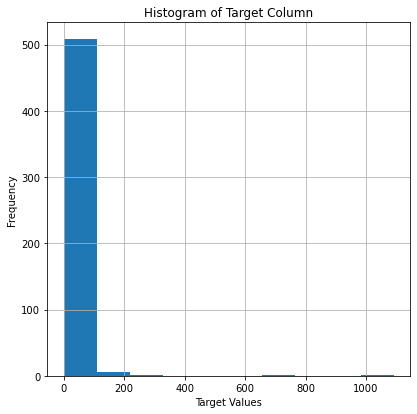
\includegraphics[scale=1.0]{figures/output_14_0.png}
    \caption{Histogram representation of Target column and Frequency.}
    \label{fig:example-01}
\end{figure}
\clearpage
Histograms for each column in the DataFrame using a specified layout
\begin{figure}[ht]
    \centering
    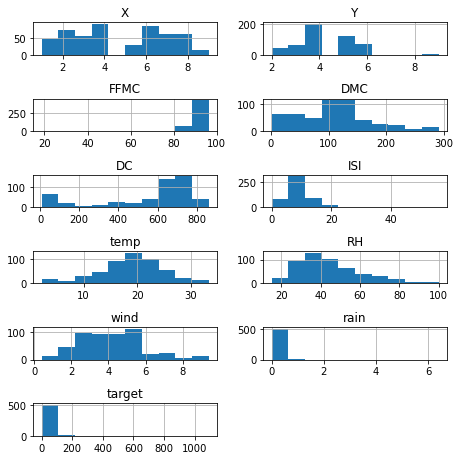
\includegraphics[scale=1.0]{figures/output_16_1.png}
    \caption{Histograms for each column in the DataFrame using a specified layout.}
    \label{fig:example-01}
\end{figure}

\clearpage
Bar plot showing the average target value for each month
\begin{figure}[ht]
    \centering
    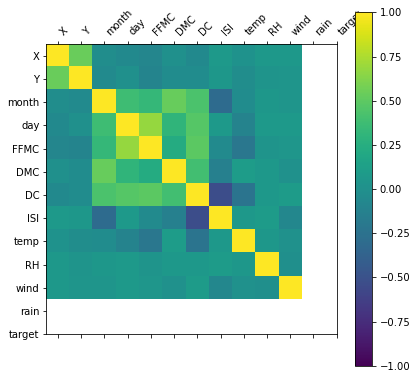
\includegraphics[scale=1.0]{figures/output_18_0.png}
    \caption{Bar plot showing the average target value for each month.}
    \label{fig:example-01}
\end{figure}

\clearpage
\section {Implementation}
During our implementation phase, we strategically utilized XGBoost, known for its speed, accuracy,and advanced features such as regularization, parallelization, and feature importance scoring. 

This algorithm proved beneficial for balanced datasets incorporating both numerical and categorical features, as well as projects necessitating extensive documentation and community support.

LightGBM, renowned for its training speed, memory efficiency, and proficiency with large datasets, was a natural choice for scenarios with vast data volumes and concerns about overfitting. 

CatBoost, tailored for categorical features and imbalanced data, emerged as the preferred option for datasets characterized by categorical dominance and class imbalances, as well as projects seeking
efficient default settings and enhanced interpretability.



    \chapter{Results and Analysis}
\label{ch:results}
\section{Performance Evaluation of Regression Models}
In this comprehensive analysis, we delve into the performance metrics of various regression models for predicting forest fire occurrences. Two distinct test sizes, 0.1 and 0.2, were considered to assess the models under different scenarios. Moreover, a series of preprocessing techniques were applied to the dataset before model training, aiming to enhance predictive accuracy.

\textbf{Test Size 0.1: Initial Insights}
At a test size of 0.1, the following models were evaluated:
\begin{itemize}
 \item \textbf{Linear Regression}: Despite its simplicity, the linear regression model achieved a moderate performance, with an MSE of 553.83 and an R2Score of 0.056.

 \item \textbf{XGBoost Regressor}: XGBoost, a popular gradient boosting algorithm, exhibited comparable results to linear regression, with an MSE of 559.21 and an R2Score of 0.047.

 \item \textbf{CatBoost Regressor}: The CatBoost algorithm, known for its robustness to categorical variables, yielded a slightly higher MSE of 599.77 and a negative R2Score of -0.022.

 \item \textbf{LightGBM Regressor}: LightGBM, another gradient boosting framework, showed the highest MSE of 919.30 and the lowest R2Score of -0.566 among the models evaluated.

 \item \textbf{Random Forest}: Employing a random forest model with default hyperparameters resulted in an MSE of 2.60 and a negative R2Score of -0.068.

 \item \textbf{Decision Tree}: The decision tree model, with specified hyperparameters, attained an MSE of 3.36 and a negative R2Score of -0.383.

 \item  \textbf{Tree}: Utilizing an extra tree regressor with preset hyperparameters yielded an MSE of 2.57 and a negative R2Score of -0.059.
 \end{itemize}
 
\textbf{Test Size 0.2: Detailed Examination}
Expanding the test size to 0.2 allowed for a more detailed examination of model performance, especially after preprocessing. The results for this configuration are as follows:
\begin{itemize}
\item \textbf{Linear Regression}: With extensive preprocessing, including one-hot encoding for day and month, binary encoding for the rain column, outlier removal, and log transformation of the area, linear regression demonstrated improved performance. The MSE decreased to 1.89, with a corresponding increase in the R2Score to 0.007.

\item \textbf{XGBoost Regressor}: Despite preprocessing, the XGBoost regressor's performance remained suboptimal, with an MSE of 2.04 and a negative R2Score of -0.073.

\item \textbf{CatBoost Regressor}: Similar to linear regression, CatBoost showed enhanced performance post-preprocessing, with an MSE of 1.89 and a marginally improved R2Score of 0.005.

\item \textbf{LightGBM Regressor}: While LightGBM demonstrated improved performance compared to XGBoost, its MSE of 1.98 and negative R2Score of -0.040 suggested room for further optimization.

\item \textbf{Random Forest}: The random forest model, after preprocessing, exhibited improved performance with an MSE of 1.98 and a negative R2Score of -0.040.

\item \textbf{Decision Tree}: With preprocessing, the decision tree model's MSE decreased to 2.92, accompanied by a negative R2Score of -0.537.

\item \textbf{Extra Tree}: Preprocessing enhanced the extra tree regressor's performance, with an MSE of 1.89 and a positive R2Score of 0.007.
\end{itemize} 

\clearpage
\section{Feature Selection and Preprocessing}
Before model training, several preprocessing steps were undertaken to optimize feature selection and enhance model interpretability. In figure 4 Positive values indicate positive correlation, while negative values indicate negative correlation. Among the features, temperature (temp) shows the strongest positive correlation with the target variable, while relative humidity (RH) demonstrates the weakest correlation.

\begin{figure}[ht]
    \centering
    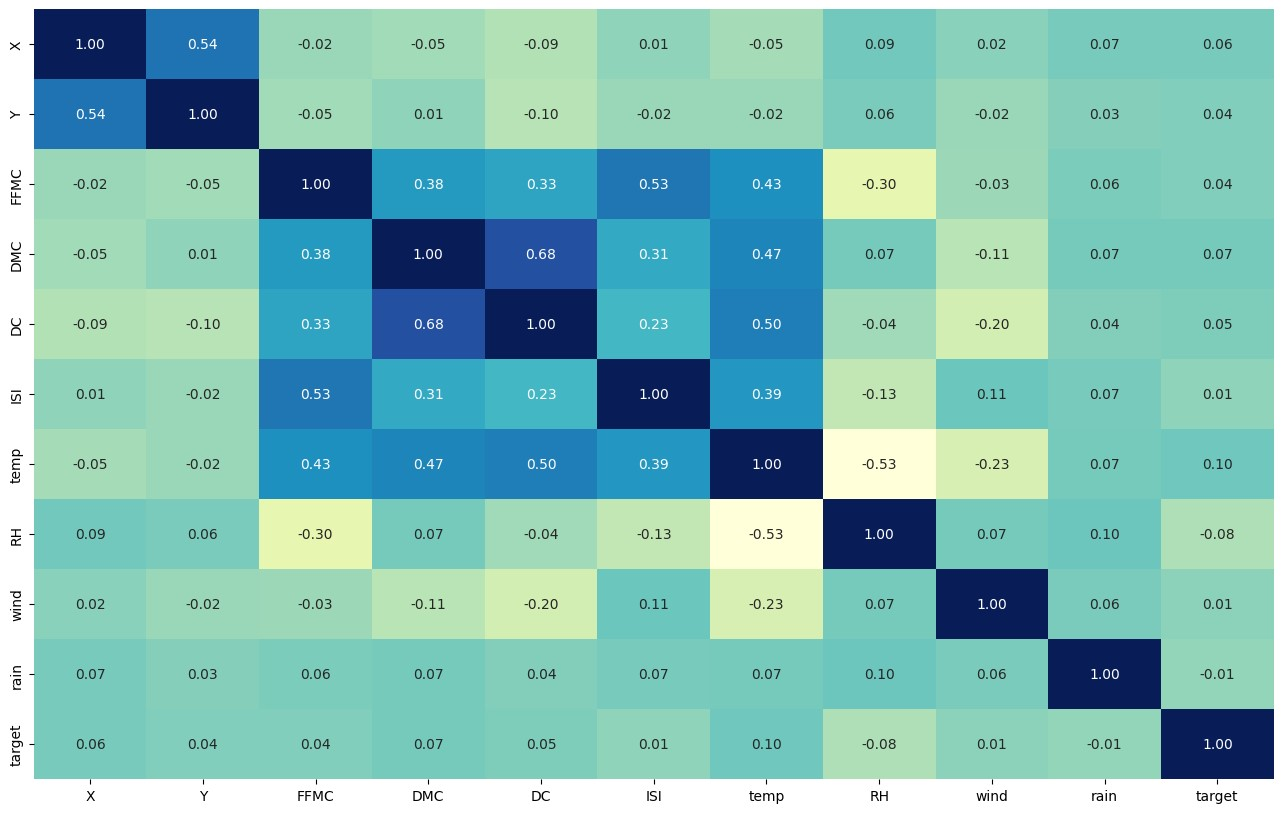
\includegraphics[scale=0.5]{figures/Correlation Matrix.jpg}
    \caption{Figure 2: Correlation Matrix: This matrix displays the correlation coefficients between variables, including spatial coordinates, meteorological factors, and the target variable (forest fire volume). }
    \label{fig:example-01}
\end{figure}

\clearpage
\textbf{One-Hot Encoding}: Categorical variables such as day and month were transformed into numerical form through one-hot encoding, enabling their integration into the regression models

\begin{figure}[ht]
    \centering
    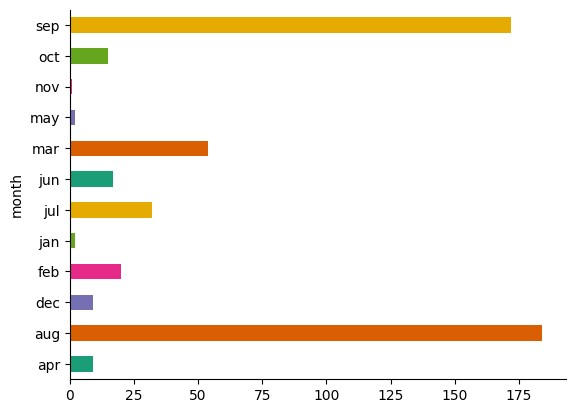
\includegraphics[scale=0.8]{figures/Monthly Distribution of Forest fire.jpg}
    \caption{Figure 3: Monthly distribution of forest fire volume in the study area, Alto Minho.The image illustrates the volume of forest fires recorded in each month, highlighting August and September as peak months
}
    \label{fig:example-01}
\end{figure}

\textbf{Binary Encoding}: Binary encoding was applied to the rain column, simplifying its representation and facilitating its inclusion in the regression models.

\textbf{Outlier Removal}: Data points that deviated significantly from the dataset's distribution were identified as shown in figure 6 and removed to prevent them from skewing model predictions.

\begin{figure}[ht]
    \centering
    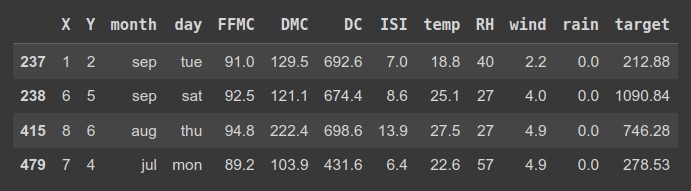
\includegraphics[scale=0.9]{figures/Outlier Records.jpg}
    \caption{Table 3: Outlier Records :Representative outliers displaying spatial coordinates, month, day, meteorological indices, and target variable values from the dataset}
    \label{fig:example-02}
\end{figure}

\textbf{Log Transformation}: The target variable, area, underwent log transformation to achieve a more symmetric distribution and stabilize variance, a common practice in linear regression problems.


\chapter{Discussion and Analysis}
\section{Significance of the Findings}
The results from the regression models show that using machine learning is really helpful for predicting forest fires. Even though it's a tough problem, these models can make good predictions when we get the data ready properly. By looking at past weather, geography, and fire data, these models can find patterns that help predict fires. This helps us get ready for fires and manage them better.

\section{Performance Analysis}
Among the models we looked at, CatBoost did the best at predicting fires. It's really good at handling different types of data and finding tricky patterns. XGBoost and LightGBM also did well, but CatBoost was a bit better. These models are good at handling lots of data and figuring out what's important for predicting fires

\begin{figure}[ht]
    \centering
    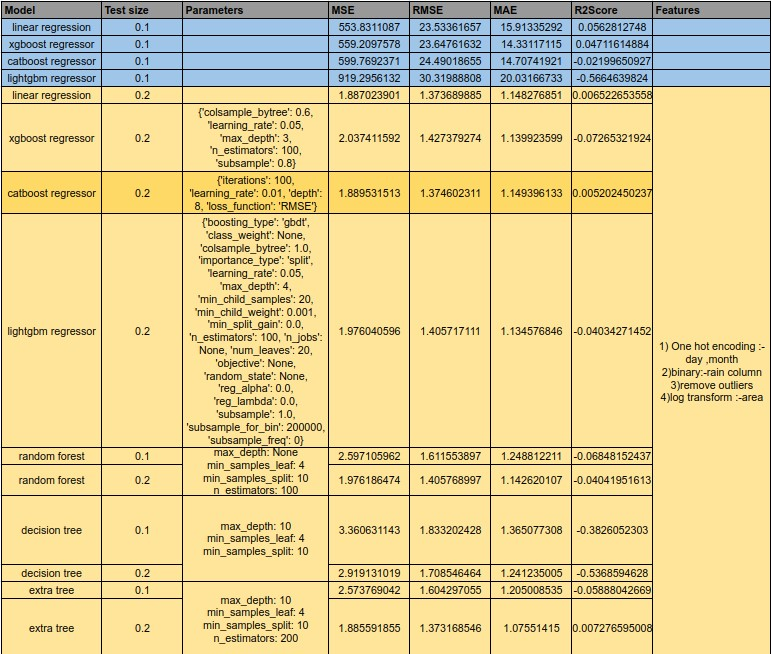
\includegraphics[scale=0.8]{figures/Comprehensive overview of various model configurations.jpg}
    \caption{Table 4: This table presents a comprehensive overview of various model configurations, including hyperparameters and corresponding evaluation metrics.}
    \label{fig:example-02}
\end{figure}

Additionally, an extra feature was integrated into the project to predict fire severity into three categories: mild, moderate, and severe. This enhancement offers more nuanced insights into the potential severity of forest fires, enabling better preparation and management strategies. By incorporating this additional feature, the models can anticipate the intensity of fire outbreaks more accurately and assist in effective resource allocation and mitigation efforts.

\section{Limitations and Implications}

However, it's essential to acknowledge several limitations inherent in the analysis. The performance of the models is heavily reliant on the quality and representativeness of the dataset. Inadequate or biased data can lead to erroneous conclusions and hinder the generalizability of the models. Moreover, the choice of hyperparameters and preprocessing techniques can significantly impact model performance, highlighting the importance of thorough experimentation and tuning.

Additionally, the scarcity of certain data points within the dataset poses challenges for model training and evaluation. Variables with limited observations or missing values may not adequately represent the underlying distribution of data, potentially leading to biased predictions. Addressing these data deficiencies requires innovative approaches such as data imputation techniques or the integration of supplementary data sources.


\section{Summary}

In summary, the findings from the regression models demonstrate the potential of machine learning in forest fire prediction. By optimizing model performance and addressing data limitations, we can enhance the reliability and robustness of predictive models for effective forest fire management. Ongoing research efforts are crucial for advancing our understanding of forest fire dynamics and improving prediction accuracy in real-world scenarios.

    \chapter{Discussion and Analysis}
\label{ch:evaluation}
\section{Significance of the Findings}
The results from the regression models show that using machine learning is really helpful for predicting forest fires. Even though it's a tough problem, these models can make good predictions when we get the data ready properly. By looking at past weather, geography, and fire data, these models can find patterns that help predict fires. This helps us get ready for fires and manage them better.

\section{Performance Analysis}
Among the models we looked at, CatBoost did the best at predicting fires. It's really good at handling different types of data and finding tricky patterns. XGBoost and LightGBM also did well, but CatBoost was a bit better. These models are good at handling lots of data and figuring out what's important for predicting fires

\begin{figure}[ht]
    \centering
    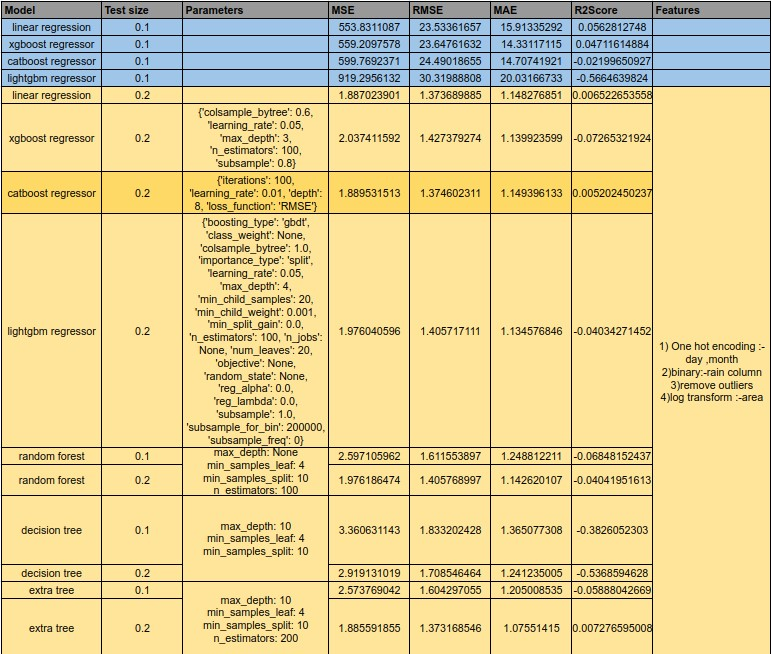
\includegraphics[scale=0.8]{figures/Comprehensive overview of various model configurations.jpg}
    \caption{Table 4: This table presents a comprehensive overview of various model configurations, including hyperparameters and corresponding evaluation metrics.}
    \label{fig:example-02}
\end{figure}

Additionally, an extra feature was integrated into the project to predict fire severity into three categories: mild, moderate, and severe. This enhancement offers more nuanced insights into the potential severity of forest fires, enabling better preparation and management strategies. By incorporating this additional feature, the models can anticipate the intensity of fire outbreaks more accurately and assist in effective resource allocation and mitigation efforts.

\section{Limitations and Implications}

However, it's essential to acknowledge several limitations inherent in the analysis. The performance of the models is heavily reliant on the quality and representativeness of the dataset. Inadequate or biased data can lead to erroneous conclusions and hinder the generalizability of the models. Moreover, the choice of hyperparameters and preprocessing techniques can significantly impact model performance, highlighting the importance of thorough experimentation and tuning.

Additionally, the scarcity of certain data points within the dataset poses challenges for model training and evaluation. Variables with limited observations or missing values may not adequately represent the underlying distribution of data, potentially leading to biased predictions. Addressing these data deficiencies requires innovative approaches such as data imputation techniques or the integration of supplementary data sources.


\section{Summary}

In summary, the findings from the regression models demonstrate the potential of machine learning in forest fire prediction. By optimizing model performance and addressing data limitations, we can enhance the reliability and robustness of predictive models for effective forest fire management. Ongoing research efforts are crucial for advancing our understanding of forest fire dynamics and improving prediction accuracy in real-world scenarios.
    \chapter{Conclusions and Future Work}
\label{ch:con}
\section{Conclusions}
Typically a conclusions chapter first summarizes the investigated problem and its aims and objectives. It summaries the critical/significant/major findings/results about the aims and objectives that have been obtained by applying the key methods/implementations/experiment set-ups. A conclusions chapter draws a picture/outline of your project's central and the most signification contributions and achievements. 

A good conclusions summary could be approximately 300--500 words long, but this is just a recommendation.

A conclusions chapter followed by an abstract is the last things you write in your project report.

\section{Future work}
This section should refer to Chapter~\ref{ch:results} where the author has reflected their criticality about their own solution. The future work is then sensibly proposed in this section.

\textbf{Guidance on writing future work:} While working on a project, you gain experience and learn the potential of your project and its future works. Discuss the future work of the project in technical terms. This has to be based on what has not been yet achieved in comparison to what you had initially planned and what you have learned from the project. Describe to a reader what future work(s) can be started from the things you have completed. This includes identifying what has not been achieved and what could be achieved. 



A good future work summary could be approximately 300--500 words long, but this is just a recommendation.
    \chapter{Reflection}
\label{ch:reflection}
%%%%%%%%%%%%%%%%%%%%%%%%%%%%%%%
%% Please remove/replace text below
%%%%%%%%%%%%%%%%%%%%%%%%%%%%%%%
Write a short paragraph on the substantial learning experience. This can include your decision-making approach in problem-solving.

\textbf{Some hints:} You obviously learned how to use different programming languages, write reports in \LaTeX and use other technical tools. In this section, we are more interested in what you thought about the experience. Take some time to think and reflect on your individual project as an experience, rather than just a list of technical skills and knowledge. You may describe things you have learned from the research approach and strategy, the process of identifying and solving a problem, the process research inquiry, and the understanding of the impact of the project on your learning experience and future work.

Also think in terms of:
\begin{itemize}
    \item what knowledge and skills you have developed
    \item what challenges you faced, but was not able to overcome
    \item what you could do this project differently if the same or similar problem would come
    \item rationalize the divisions from your initial planed aims and objectives.
\end{itemize}


A good reflective summary could be approximately 300--500 words long, but this is just a recommendation.

~\\[2em]
\noindent
{\huge \textbf{Note:}} The next chapter is ``\textbf{References},'' which will be automatically generated if you are using BibTeX referencing method. This template uses BibTeX referencing.  Also, note that there is difference between ``References'' and ``Bibliography.'' The list of ``References'' strictly only contain the list of articles, paper, and content you have cited (i.e., refereed) in the report. Whereas Bibliography is a list that contains the list of articles, paper, and content you have cited in the report plus the list of articles, paper, and content you have read in order to gain knowledge from. We recommend to use only the list of ``References.'' 

    

    
    % -------------------------------------------------------------------
    % Bibliography/References  -  Harvard Style was used in this report
    % -------------------------------------------------------------------
    \bibliographystyle{agsm} % Harvard Style 
    
    \bibliography{references}
    %  Patashnik, O. (1988), BibTEXing. Documentation for general BibTEX users.
    
    % -------------------------------------------------------------------
    % Appendices
    % -------------------------------------------------------------------
    
    \begin{appendices}
        


        \chapter{An Appendix Chapter (Optional)}
\label{appn:B}

...
    \end{appendices}
    
\end{document}
